\section{Module 10. Upsampling}

Image spatial resolution is limited by several factors. There are for example time of acquisition, organ motions, signal to noise ratio or medical equipment which do not meet the specialized requirements. Specialists usually make relatively small number of 2-D slices. It takes less time but it also results in large slice thickness and spacing between slices. Another example are voxel-wise analysis. The method requires all image volumes of one subject to be analysed in one space. If they are not acquired from the same location (because of the organ motions) the interpolation must be involved.

Interpolation is a method of constructing new points based on the
existing ones. In other words finding a value of a new point in High
Resolution (HR) image based on points in Low Resolution (LR) pictures.

In classical interpolation techniques pixels in LR data $y$ can be
related to the corresponding $x$ values of HR data:
\centerline {$y_{p}=\frac{1}{N}\sum_{i=1}^{N}x_{i}+n$, where }
\newline $y_{p}$ is the pixel of LR image at location $p$, \newline $x_{i}$ is each one of the $N$ High Resolution pixels contained within this
LR pixel,
\newline $n$ is some additive noise.

In classical interpolation techniques the High Resolution pixels $x$ are calculated as weighted average of existing LR pixels $y$.
\newline \centerline{$x_{i}=\frac{1}{M}\sum_{i=1}^{M}w_{ij}*y_{j}$, where}
\newline $w$ are weighted calculated as Euclidean distance between $M$ existing surrounding LR pixels and the coordinates of new ones.   

The biggest problem is that to find High Resolution data from the
Low Resolution values. Unfortunately, there is an infinite number
of values that meet that condition. Interpolation methods can be divided
into three basic techniques.

The first group are the most common ones, like linear or spline-based
interpolation. These techniques assume that it is possible to count
the value of a new point by determination some kind of generic function.
The main disadvantage is that they are correct only for images of
homogeneous regions. As is well known, brain consists of grey substance,
white substance and cerebral spinal fluid, so above-mentioned methods
are not appropriate for MRI images interpolation. The second one is
Super Resolution technique. It is commonly used to increase image
resolution on functional MRI (fMRI) and Diffusion Tensor Imaging (DTI).
The method is based on acquisition of multiple Low Resolution (LR)
images of the same object. It is time consuming and not adequate for
clinical applications.

The last but not least method is non-local patch-based technique which is based on self-similarity of a single image. It is possible to improve resolution by extracting information from a single image instead of acquiring several pictures.

First of all, there is a constraint which says that the original LR image has to be equal to the downsampled version $X$ of the reconstructed image. It is named subsampling consistency constraint which is written as:
\newline \centerline{$y_{p}-\frac{1}{N}\sum{i=1}^{N}X_{i}=0$}
\newline To make the above equation real, the noise has to be removed. The presence of noise has to be minimalized on the LR image by applying a filter, for example MNLM3D filter for 3D MR images based on Non-Local Means filter. The filter removes the noise effectively without affecting the image structure. 


The aim of this module is to increase MRI image resolution by upsampling.
The input data is a single 320x240 image. After the processing it
is going to be twice as big. To be more specific 640x480 pixels. The
process can be named as double upsampling.

\begin{figure}[H]
\centering{}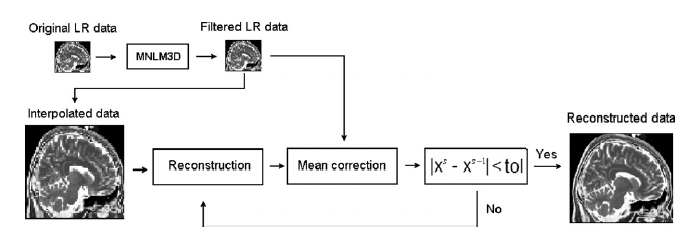
\includegraphics[scale=0.7]{Module9_1}\caption{Diagram of the patch-based non-local algorithm \cite{9art1}}. 
\label{fig: Module9_1}
\end{figure}

In a nutshell, the first step of the algorithm is to divide every pixel of LR image into more pixels. Then the patch is designed. It is a rectangle which will be the area of interest. The pixels that are inside the area are taken into account during calculation the values of new points.
After that an appropriate estimator is used to correctly calculate the values of new pixels. Every pixel has to be classified into one of three groups (grey substance, white substance or cerebral spinal fluid).

In order to show how the algorithm is designed the following pictured were generated using exemplary data. At the beginning there is an image 256x256 pixels. 

\begin{figure}[H]
\centering{}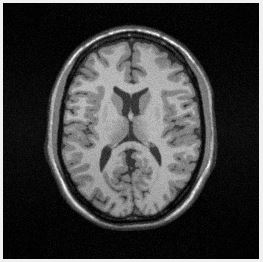
\includegraphics[scale=0.7]{Module9_2}\caption{DICOM Low Resolution image 256x256}. 
\label{fig: Module9_2}
\end{figure}

The first step is to add new pixels to increase the resolution M times horizontally and N times vertically. The pixels are equal to zero. After this process an appropriate estimator has to be chosen to make a decision about the values of new points.

\begin{figure}[H]
\centering{}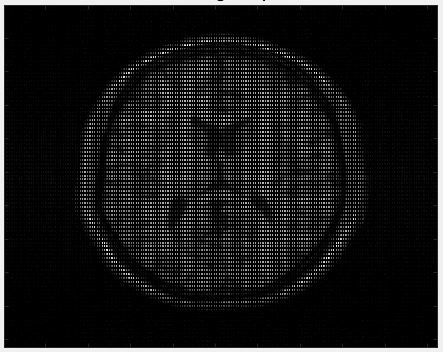
\includegraphics[scale=0.7]{Module9_3}\caption{DICOM image with new points with N=2 and M=2}. 
\label{fig: Module9_3}
\end{figure}

Patch-based non-local regularization is used to reconstruct new voxels. The voxel under study is reconstruced using all similar voxels which are placed inside the patch. Contrary to classical techniques which use local neighbourhood of the reconstructed voxel, the proposed method uses the only relevant information, the context of the voxel.

Another step in the algorithm diagram (Fig. \ref{fig: Module9_1}) is mean correction. It has to be applied to ensure that the downsampled reconstructed HR $X$ image is equal to the original $y$ LR one. Thus the local mean value of $X$ fits with the value of the $y$ by adding the corresponding offset.

\centerline{$X=X+NN*(D(X)-y)$, where}

$D$ is an operator that downsamples HR into original LR,
\newline $NN$ is a Nearest Neighbour operator that interpolates LR image to HR.

The Regularization and Correction steps are repeated until no important difference between two consecutive reconstructions. Tolerance is determined by Mean Absolute Difference .

\hfill{}\\
\textbf{List of References}\\
\cite{9art1}
\cite{9art2}
